% Bolometro Simulato - Presentazione
% Tor Vergata Engineering Beamer Template

\documentclass[aspectratio=169]{beamer}

\usepackage[
    title={Simulazione di un Bolometro},
    subtitle={Modello diretto, rumore e sorgente a corpo nero},
    event={Laboratorio di Fisica del Plasma},
    author={F.~Rosi},
    longauthor={Federico Rosi},
    email={federicorosi072@gmail.com},
    institute={Univ. di Roma ``Tor Vergata''},
    longinstitute={Universit\`a degli Studi di Roma ``Tor Vergata''},
    department={Ingegneria},
    researchgroup={},
    date={Maggio 2026}
]{utvengbeamer}

\usepackage{amsmath}
\usepackage{graphicx}
\usepackage{booktabs}
\usepackage{siunitx}

\begin{document}

% --- Title page ---
\frame{\titlepage}

% --- Table of contents ---
\begin{frame}
\frametitle{Sommario}
\tableofcontents
\end{frame}

% --- Sections ---
% =====================================================================
%  BLOCCO 1 --- Modello fisico del bolometro e modello diretto
% =====================================================================

\section{Blocco 1 --- Modello diretto}

% --- Slide: cos'è un bolometro ---
\begin{frame}
\frametitle{Cos'\`e un bolometro?}

Un \textbg{bolometro} \`e un sensore termico che misura la potenza
irradiata assorbita convertendola in una variazione di resistenza elettrica.

\vspace{0.4em}
\begin{columns}[T]
  \begin{column}{0.55\textwidth}
    \textbf{Principio di funzionamento:}
    \begin{enumerate}
      \item La radiazione incidente deposita potenza $P$ sull'assorbitore
      \item L'assorbitore si riscalda: $\Delta T = P / G$
      \item La resistenza varia: $\Delta R = R_0\,\alpha\,\Delta T$
      \item Il circuito di bias converte $\Delta R$ in tensione: $\Delta V = I_\text{bias}\,\Delta R$
    \end{enumerate}
  \end{column}
  \begin{column}{0.42\textwidth}
    \textbf{Parametri fondamentali:}
    \begin{itemize}
      \item $R_0 = \SI{100}{\ohm}$ \quad resistenza a freddo
      \item $\alpha = \SI{3.9e-3}{\per\kelvin}$ \quad TCR del Pt
      \item $G = \SI{1e-4}{\watt\per\kelvin}$ \quad conduttanza termica
      \item $I_\text{bias} = \SI{1}{\milli\ampere}$ \quad corrente di polarizzazione
      \item $T_0 = \SI{300}{\kelvin}$ \quad temperatura base
    \end{itemize}
  \end{column}
\end{columns}

\end{frame}

% --- Slide: catena segnale ---
\begin{frame}
\frametitle{Catena del segnale --- Blocco~1}

La catena di trasduzione dal segnale fisico alla tensione di uscita:

\vspace{0.6em}
\[
  P \;\longrightarrow\;
  \Delta T = \frac{P}{G} \;\longrightarrow\;
  \Delta R = R_0\,\alpha\,\Delta T \;\longrightarrow\;
  \Delta V_\text{ideal} = I_\text{bias}\,\Delta R
\]

\vspace{0.5em}
Sostituendo esplicitamente:
\[
  \boxed{\Delta V_\text{ideal} = \frac{I_\text{bias}\,R_0\,\alpha}{G}\,P
         \;=\; S \cdot P}
\]

dove la \textbf{sensibilit\`a} vale $S = I_\text{bias}\,R_0\,\alpha / G
= \SI{3.9}{\volt\per\watt}$.

\vspace{0.4em}
\begin{block}{Saturazione}
  \begin{itemize}
    \item \textbr{Termica}: $\Delta T > \Delta T_\text{max} = \SI{50}{\kelvin}
          \;\Rightarrow\; P_\text{sat} = G\,\Delta T_\text{max} = \SI{5e-3}{\watt}$
    \item \textbr{Elettrica}: $|\Delta V_\text{ideal}| > V_\text{sat} = \SI{1}{\volt}
          \;\Rightarrow\; P_\text{sat,el} \approx \SI{0.26}{\watt}$
  \end{itemize}
  La saturazione termica interviene \textbf{prima}: $\Delta V = \pm V_\text{sat}$ se saturato.
\end{block}

\end{frame}

% --- Slide: risultati numerici ---
\begin{frame}
\frametitle{Risultati numerici --- Blocco~1}

Risposta del bolometro per cinque livelli di potenza di riferimento:

\vspace{0.5em}
\begin{center}
\begin{tabular}{ccccl}
  \toprule
  $P$~[W] & $\Delta T$~[K] & $\Delta V_\text{ideal}$~[V] & $\Delta V$~[V] & Regime \\
  \midrule
  \num{1e-9} & \num{1e-5}  & \num{3.9e-6}  & \num{3.9e-6}  & OK \\
  \num{1e-7} & \num{1e-3}  & \num{3.9e-4}  & \num{3.9e-4}  & OK \\
  \num{1e-5} & \num{0.1}   & \num{3.9e-2}  & \num{3.9e-2}  & OK \\
  \num{1e-3} & \num{10}    & \num{3.9}     & \num{3.9}     & OK \\
  \num{1e-1} & \num{1000}  & \num{390}     & \num{1.0}     & \textbr{SATURATO} \\
  \bottomrule
\end{tabular}
\end{center}

\vspace{0.4em}
\small
$P_\text{sat} = V_\text{sat}\,G\,/\,(I_\text{bias}\,R_0\,\alpha)
= \SI{2.56e-1}{\watt}$ \quad (saturazione elettrica)\\
Saturazione termica: $P = G\,\Delta T_\text{max} = \SI{5e-3}{\watt}$
\quad $\Rightarrow$ \textbg{termica domina}

\end{frame}

% =====================================================================
%  BLOCCO 2 --- Rumore e sensibilità
% =====================================================================

\section{Blocco 2 --- Rumore e NEP}

% --- Slide: modello di rumore ---
\begin{frame}
\frametitle{Modello di rumore --- Blocco~2}

Il segnale misurato \`e affetto da un \textbg{rumore gaussiano generico}
che modella tutti i contributi (Johnson, amplificatore, ADC, \ldots):

\[
  \Delta V_\text{noisy} = \Delta V + \varepsilon, \qquad
  \varepsilon \sim \mathcal{N}(0,\, V_\text{noise}^2)
\]

con $V_\text{noise} = \SI{1e-5}{\volt}$ (floor di rumore totale).

\vspace{0.4em}
\begin{columns}[T]
  \begin{column}{0.48\textwidth}
    \textbf{Rapporto segnale-rumore:}
    \[
      \mathrm{SNR} = \frac{|\Delta V|}{V_\text{noise}}
    \]
    \begin{itemize}
      \item $\mathrm{SNR} \geq 1$: segnale \textbg{ricostruibile}
      \item $\mathrm{SNR} < 1$: \textbr{dominato dal rumore}
    \end{itemize}
  \end{column}
  \begin{column}{0.48\textwidth}
    \textbf{Potenza equivalente di rumore (NEP):}
    \[
      \mathrm{NEP} = \frac{V_\text{noise}}{S}
                   = \frac{V_\text{noise}\,G}{I_\text{bias}\,R_0\,\alpha}
    \]
    Con i parametri nominali:
    \[
      \mathrm{NEP} \approx \SI{2.56e-6}{\watt}
    \]
  \end{column}
\end{columns}

\end{frame}

% --- Slide: tre regimi operativi ---
\begin{frame}
\frametitle{Tre regimi operativi}

\begin{columns}[T]
  \begin{column}{0.33\textwidth}
    \centering
    \textbr{\textbf{Rumore dominante}}\\[0.3em]
    $P < \mathrm{NEP}$\\[0.2em]
    $\mathrm{SNR} < 1$\\[0.2em]
    Il segnale \`e sepolto nel rumore. La misura non \`e affidabile.
  \end{column}
  \begin{column}{0.33\textwidth}
    \centering
    \textbg{\textbf{Ricostruibile}}\\[0.3em]
    $\mathrm{NEP} \leq P < P_\text{sat}$\\[0.2em]
    $\mathrm{SNR} \geq 1$\\[0.2em]
    Il bolometro opera linearmente. $P$ \`e stimabile da $\Delta V$.
  \end{column}
  \begin{column}{0.30\textwidth}
    \centering
    \textcolor{orange}{\textbf{Saturato}}\\[0.3em]
    $P \geq P_\text{sat}$\\[0.2em]
    $|\Delta V| = V_\text{sat}$\\[0.2em]
    L'uscita \`e bloccata a $\pm\SI{1}{\volt}$. Solo un lower bound su $P$.
  \end{column}
\end{columns}

\vspace{0.6em}
\begin{alertblock}{Dinamica del bolometro}
  Il \textbf{range dinamico} utile \`e
  $[\mathrm{NEP},\, P_\text{sat}] =
  [\SI{2.56e-6}{\watt},\; \SI{5e-3}{\watt}]$,
  ovvero circa \textbg{3 decadi} in potenza.
\end{alertblock}

\end{frame}

% --- Slide: grafico blocchi 1-2 ---
\begin{frame}
\frametitle{Grafici --- Modello diretto e rumore}

\begin{center}
  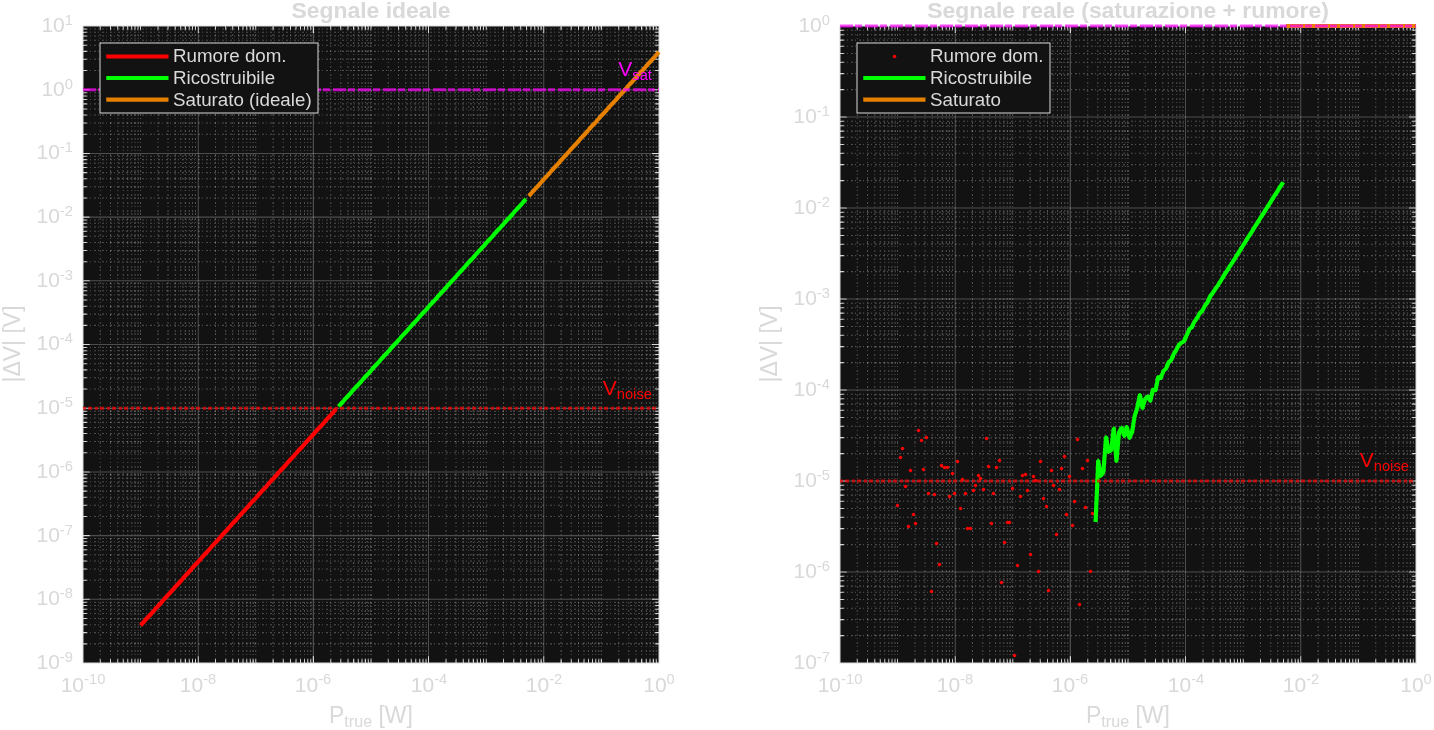
\includegraphics[width=0.90\textwidth]{blocchi_1_2_risultati.png}
\end{center}

\vspace{-0.3em}
\small
\textit{Sinistra}: segnale ideale $|\Delta V_\text{ideal}|$ vs $P$.
\textit{Destra}: segnale reale con saturazione e rumore gaussiano.
I colori indicano il regime: \textbr{rosso} = rumore dominante,
\textbg{verde} = ricostruibile, \textcolor{orange}{arancio} = saturato.

\end{frame}

% =====================================================================
%  BLOCCO 3 --- Radiazione di corpo nero e potenza assorbita
% =====================================================================

\section{Blocco 3 --- Sorgente a corpo nero}

% --- Slide: contesto fisico ---
\begin{frame}
\frametitle{Contesto fisico --- Plasma da fusione}

Il bolometro \`e impiegato per misurare la \textbg{radiazione totale}
emessa dal plasma in un tokamak.

\vspace{0.4em}
\begin{columns}[T]
  \begin{column}{0.55\textwidth}
    \textbf{Sorgente ipotizzata:}
    \begin{itemize}
      \item Corpo nero a temperatura del plasma di bordo
      \item $T_\text{source} = \SI{85}{\electronvolt}
            \approx \SI{9.9e5}{\kelvin}$
      \item Banda di frequenza: NIR $\to$ raggi~X
        \[
          f \in [3\times10^{14},\; 3\times10^{18}]\;\si{\hertz}
        \]
      \item Lunghezze d'onda: $\lambda \in [\SI{0.1}{\nano\meter},\; \SI{1000}{\nano\meter}]$
    \end{itemize}
  \end{column}
  \begin{column}{0.42\textwidth}
    \textbf{Obiettivo del Blocco 3:}
    \begin{enumerate}
      \item Calcolare la radianza spettrale $B(f,T)$
      \item Pesare con l'assorbanza del sensore $A(f)$
      \item Integrare su tutte le frequenze:\\
            $P_\text{abs} = \int B\,A\,\mathrm{d}f$
      \item Calcolare il rapporto\\
            $\eta = P_\text{abs} / P_\text{emit}$
      \item Studiare $\eta(T)$ al variare di $T$
    \end{enumerate}
  \end{column}
\end{columns}

\end{frame}

% --- Slide: formula di Planck ---
\begin{frame}
\frametitle{Radianza spettrale di Planck}

La \textbg{radianza spettrale} di un corpo nero a temperatura $T$ \`e:

\[
  B(f, T) = \frac{2\,h\,f^3}{c^2}
             \cdot \frac{1}{\exp\!\left(\dfrac{h\,f}{k_B\,T}\right) - 1}
  \quad \left[\si{\watt\per\meter\squared\per\steradian\per\hertz}\right]
\]

\vspace{0.3em}
\begin{columns}[T]
  \begin{column}{0.48\textwidth}
    \textbf{Costanti fisiche:}
    \begin{itemize}
      \item $h = \SI{6.626e-34}{\joule\second}$
      \item $c = \SI{3e8}{\meter\per\second}$
      \item $k_B = \SI{1.381e-23}{\joule\per\kelvin}$
    \end{itemize}
  \end{column}
  \begin{column}{0.48\textwidth}
    \textbf{Implementazione MATLAB:}
    \begin{itemize}
      \item 500 punti in \texttt{logspace} su $[3\times10^{14}, 3\times10^{18}]$\,Hz
      \item Integrazione numerica con la regola dei trapezi:
        \[
          P_\text{abs} = \int B(f,T)\,A(f)\,\mathrm{d}f
                       \approx \sum_i \Delta f_i\,B_i\,A_i
        \]
    \end{itemize}
  \end{column}
\end{columns}

\end{frame}

% --- Slide: assorbanza del platino ---
\begin{frame}
\frametitle{Assorbanza spettrale del platino}

Il sensore in platino non assorbe uniformemente su tutta la banda.
L'\textbg{assorbanza} $A(f) \in [0,1]$ \`e modellata con 7 punti chiave
e interpolazione lineare in spazio log-log:

\vspace{0.3em}
\begin{center}
\begin{tabular}{lc}
  \toprule
  Frequenza $f$~[Hz] & $A(f)$ \\
  \midrule
  $3\times10^{14}$ (NIR)     & 0.20 \\
  $6\times10^{14}$ (Vis.)    & 0.30 \\
  $1.5\times10^{15}$ (UV)    & 0.50 \\
  $3\times10^{15}$ (UV vuoto)& 0.65 \\
  $3\times10^{16}$ (EUV)     & 0.80 \\
  $3\times10^{17}$ (Molli~X) & 0.95 \\
  $3\times10^{18}$ (Duri~X)  & 0.99 \\
  \bottomrule
\end{tabular}
\end{center}

\vspace{0.2em}
\small
Il platino \`e trasparente nell'IR e quasi opaco ai raggi~X, comportamento
tipico dei metalli a film sottile usati nei bolometri da fusione.

\end{frame}

% --- Slide: risultati Planck + assorbanza ---
\begin{frame}
\frametitle{Risultati --- Radianza, assorbanza e integrando}

\begin{center}
  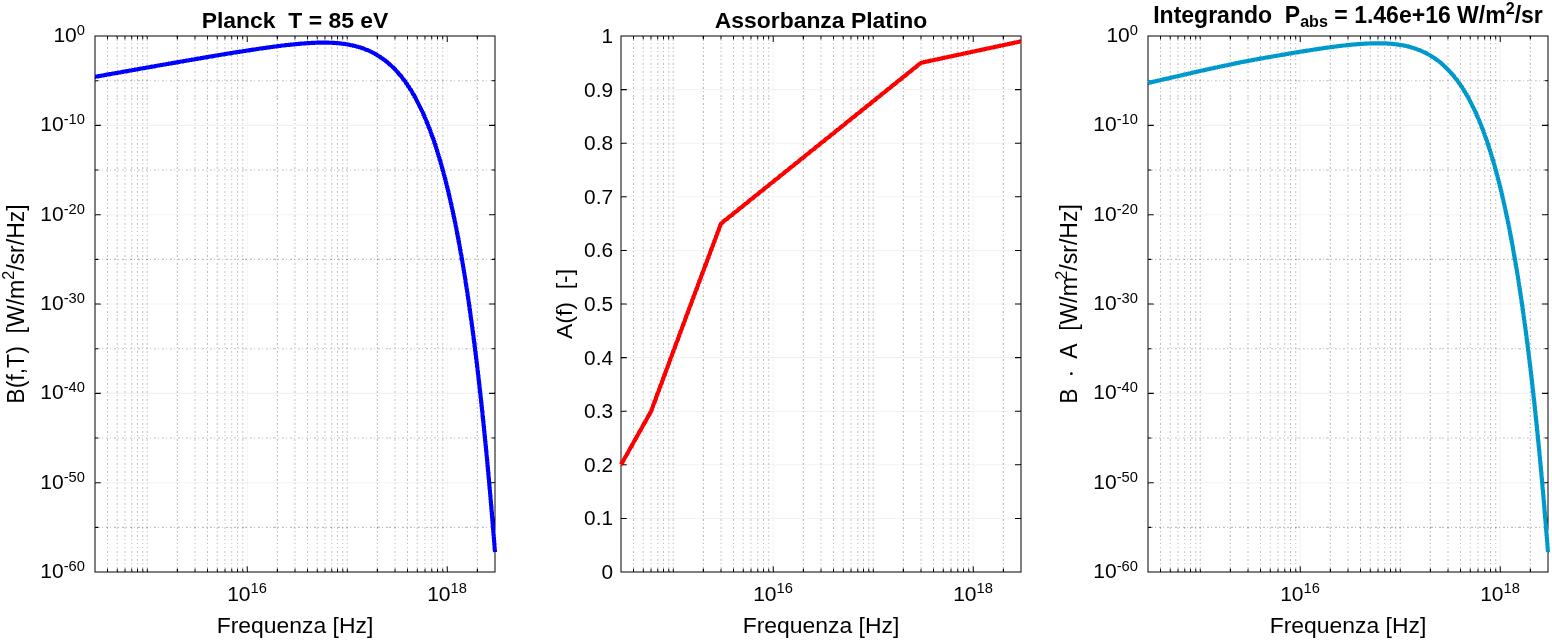
\includegraphics[width=0.92\textwidth]{blocco3_risultati.png}
\end{center}

\vspace{-0.3em}
\small
\textit{Sinistra}: $B(f,T)$ del corpo nero a $T = \SI{85}{\electronvolt}$.
\textit{Centro}: assorbanza $A(f)$ del platino.
\textit{Destra}: integrando $B(f)\cdot A(f)$ e potenza assorbita
$P_\text{abs} = \int B\,A\,\mathrm{d}f$.

\end{frame}

% --- Slide: potenza assorbita risultato numerico ---
\begin{frame}
\frametitle{Potenza assorbita --- risultato numerico}

A $T_\text{nom} = \SI{85}{\electronvolt}$, l'integrazione numerica d\`a:

\vspace{0.3em}
\begin{center}
\begin{tabular}{lrl}
  \toprule
  Grandezza & Valore & Unit\`a \\
  \midrule
  $P_\text{emit} = \int B\,\mathrm{d}f$ & dipende da $T$ & W/m$^2$/sr \\
  $P_\text{abs}  = \int B\cdot A\,\mathrm{d}f$ & $< P_\text{emit}$ & W/m$^2$/sr \\
  $\eta = P_\text{abs}/P_\text{emit}$ & vedi tabella & -- \\
  \bottomrule
\end{tabular}
\end{center}

\vspace{0.4em}
Variazione intorno a $T_\text{nom}$ con passo $\Delta T = \SI{10}{\electronvolt}$:

\vspace{0.2em}
\begin{center}
\small
\begin{tabular}{ccc}
  \toprule
  $T$~[eV] & $\eta = P_\text{abs}/P_\text{emit}$~[\%] & Nota \\
  \midrule
  55  & (minimo) & spettro spostato verso NIR \\
  \textbg{85}  & \textbg{(nominale)} & \textbg{punto di lavoro} \\
  115 & (massimo) & spettro spostato verso X \\
  \bottomrule
\end{tabular}
\end{center}

\vspace{0.3em}
\small
Il rapporto $\eta$ \textbg{cresce con $T$}: a temperature pi\`u elevate
lo spettro di Planck si sposta verso frequenze pi\`u alte, dove $A(f)$
del platino \`e maggiore (legge di Wien: $f_\text{max} \propto T$).

\end{frame}

% --- Slide: efficienza assorbimento vs T ---
\begin{frame}
\frametitle{Efficienza di assorbimento vs temperatura}

\begin{center}
  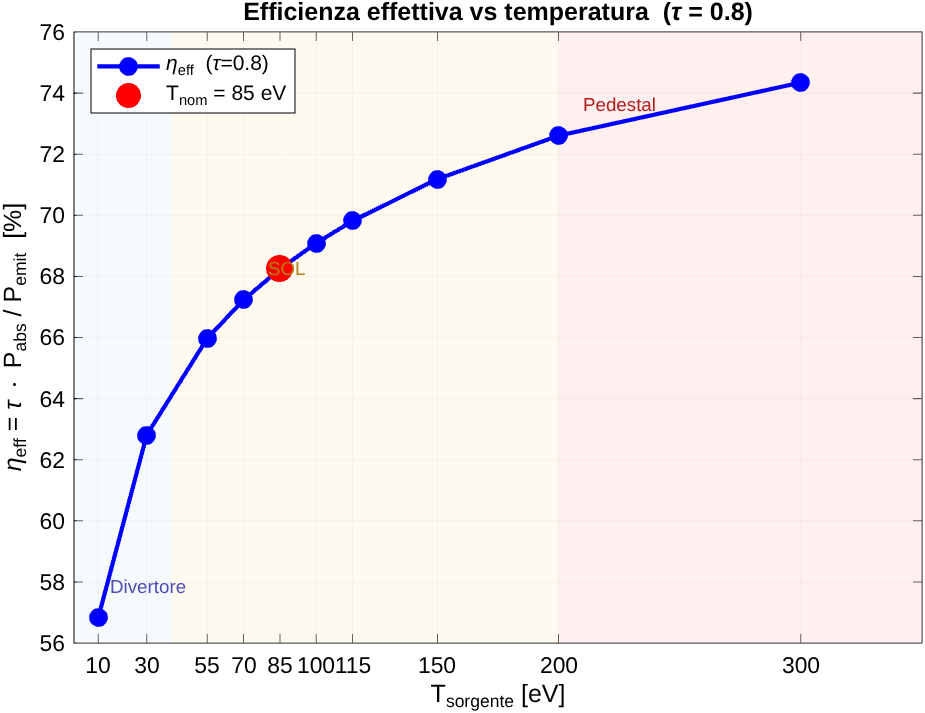
\includegraphics[width=0.72\textwidth]{blocco3_assorbimento.png}
\end{center}

\vspace{-0.3em}
\small
Il punto rosso indica $T_\text{nom} = \SI{85}{\eV}$.
La curva \`e monotona crescente: a temperature pi\`u alte il picco
dello spettro di Planck si sposta verso l'EUV/raggi~X dove il platino
assorbe di pi\`u. Il bolometro \`e quindi \textbg{pi\`u sensibile}
(a parit\`a di geometria) quando misura plasmi pi\`u caldi.

\end{frame}

% --- Slide: conclusioni ---
\begin{frame}
\frametitle{Conclusioni}

\begin{columns}[T]
  \begin{column}{0.55\textwidth}
    \textbf{Blocco 1 --- Modello diretto}
    \begin{itemize}
      \item Catena lineare $P \to \Delta T \to \Delta R \to \Delta V$
      \item Saturazione termica domina a $P_\text{sat} = \SI{5}{\milli\watt}$
    \end{itemize}

    \vspace{0.4em}
    \textbf{Blocco 2 --- Rumore}
    \begin{itemize}
      \item Rumore gaussiano $V_\text{noise} = \SI{10}{\micro\volt}$
      \item $\mathrm{NEP} \approx \SI{2.56}{\micro\watt}$
      \item Range dinamico $\approx 3$ decadi
    \end{itemize}
  \end{column}
  \begin{column}{0.42\textwidth}
    \textbf{Blocco 3 --- Corpo nero}
    \begin{itemize}
      \item Spettro di Planck a $T = \SI{85}{\electronvolt}$
      \item Assorbanza Pt da NIR a raggi~X
      \item $\eta = P_\text{abs}/P_\text{emit}$ cresce con $T$
      \item Il bolometro in Pt \`e pi\`u efficiente\\
            per plasmi pi\`u caldi
    \end{itemize}

    \vspace{0.4em}
    \begin{block}{Risultato chiave}
      La legge di Wien sposta il picco verso le X
      al crescere di $T$: il platino assorbe meglio
      l\`i, quindi $\eta(T)$ \`e crescente.
    \end{block}
  \end{column}
\end{columns}

\end{frame}


\end{document}
